\documentclass[12pt,fleqn]{article}\usepackage{../common}
\begin{document}
Ders 2

Bir diferansiyel denklemle baslayip cozebilecegimiz bir ayriksal (discrete)
probleme nasil ulasiriz? Ikinci turevi iceren basit bir diferansiyel
denkleme bakalim

\[ -\frac{d^2u}{dx^2} = f(x) \]

\[ u(0) = 0, \ u(1) = 0 \]

Eksi isareti var cunku ikinci turevler negatif kesin (negative definite)
seylerdir ve eksi isareti bu durumu telafi etmek icin, onu pozitif kesin
hale cevirmek icin konuldu. Ayrica dikkat edersek s�n�r (boundary) sartlari
var, her iki ucta da fonksiyona sifir degeri vermisiz, her iki ucta da onu
``sabitlemisiz''. Dikkat edelim, bu baslangic deger probleminden farkli,
$u$, $x$'in bir fonksiyonu, $t$ yani zamanin degil. Diyelim ki bu problem
iki tarafi sabitlenmis bir elastik cubugu temsil ediyor, $f(x)$ cubuk
uzerindeki her $x$ noktasindaki yuku gosteriyor. Bu derste $f(x) = 1$
alacagiz, yani

\[ -\frac{d^2u}{dx^2} = 1 \]

Amacimiz bir diferansiyel denklem alip, onu ayriksal olarak temsil edebilmek, yani
soyle

\[ \frac{-u_{i+1}+2u_i - u_{i-1}}{(\Delta x)^2} = f(x_i)\]

Bu denklem ikinci farkliliklari (second difference) gosteriyor. 

Diferansiyelden (differential) farkliliklara (differences) gecisin birkac
yontemi olabilir. 

Birinci Farkliliklar (Ileri Dogru)

\[ \Delta_Fu = \frac{u(x+h)-u(x)}{h} \]

Ayriksal: $(u_{i+1} - u_{i}) / h$

Birinci Farkliliklar (Geriye Dogru)

\[ \Delta_Bu = \frac{u(x)-u(x-h)}{h} \]

Ayriksal: $(u_{i-1} - u_{i}) / h$

Birinci Farkliliklar (Ortalanmis)

\[ \Delta_Cu = \frac{u(x+h)-u(x-h)}{2h} \]

Ayriksal: $(u_{i+1} - u_{i-1}) / h$

Bunlar Calculus'tan hatirlanabilecek seyler, fakat burada $h$ limitte
sifira dogru gitmiyor. Hesapsal dunyada $h$ bizim belirledigimiz bir
mesafe, belki $1$, belki $0.1$. O kadar bir hesapsal adim atmayi biz
seciyoruz, her sey ayriksal. 

Ayrica Calculus'ta hep $\Delta_F u$ gosterilir ve yaklasiksal olarak tureve
esittir yani $u'(x)$. Geriye adim da vardir, hesapsal olarak ileri adim
kadar iyidir, ve o da asagi yukari tureve esittir. Cok onemli bir farklilik
hesabi ise ortalanmis (centered) olandir, bu hesap ileri ve geri
farkliliklarin ortalamasidir, ayni sekilde asagi yukari tureve esittir.

Bastaki denklemimize birinci turevi dahil etmedik, cunku birinci turevler
anti-simetriktir. 

Birinci farkliliklar yontemine donelim, tureve ne kadar yakindirlar? 

Birinci Farkliliklar (Ileri Dogru)

\[ \Delta_Fu  \approx u'(x) + O(h) \]

Birinci Farkliliklar (Geriye Dogru)

\[ \Delta_Bu \approx u'(x) + O(h)\]

Birinci Farkliliklar (Ortalanmis)

\[ \Delta_Cu  \approx u'(x) + O(h^2)\]

$O(h)$ $h$'ye oranli (order of $h$) anlamina gelir, gercek degerden
``kesilip atilmis fark'' oldugunu farz edelim. Ortalama icin niye $O(h^2)$?
Hesabi yapalim. Taylor serilerinin ne oldugunu hatirlayalim ve $u(x+h)$
acilimini yapalim. Dikkat, ayriksal formla degil, surekli fonksiyonla
calisiyoruz, surekli fonksiyon uzerinde ``ayriksal bir adim'' atilinca ne
olacagini bulmaya calisiyoruz, bu sekilde surekli formatta, cebirsel bir
kural elde etmeye ugrasiyoruz.

\[ u(x+h) = u(x)+hu'(x)+\frac{h^2}{2}u''(x) + \frac{h^3}{6}u'''(x) ...\]

Taylor acilimlarinda ve hesapsal bilimde ikinci seviye kesinlik (accuracy)
cogunlukla yeterli oluyor. Hesapsal kodlari gelistirirken, test ederken
tipik olarak birinci seviyede baslanir, ve nihai urun, sonuc ortami
(production) icin 2. seviye eklenir. Devam edelim, geriye dogru:
\[ u(x-h) = u(x)-hu'(x)+\frac{h^2}{2}u''(x) - \frac{h^3}{6}u'''(x) + ...\]

Ortalanmis farklilik icin iki formulu birbirinden cikartiriz, ve $2h$'ye
boleriz.
\[ u(x+h)-u(x-h) = 2hu'(x) + \frac{h^3}{3}u'''\]

Iki tarafi $2h$'ye bolelim

\[ \frac{u(x+h)-u(x-h)}{2h} = u'(x) + \frac{h^2}{6}u'''\]

Goruyoruz ki ortalama farklilik dogru turevi $u'$ esitligin saginda
veriyor, ve $h^2$ terimine bakarak yaklasikligin, hatanin ikinci seviyede
oldugunu anliyoruz. 

Turevlerin yerine farklilik gecirirken secenekler bunlar. Elimizde 3
secenek var, ve cogunlukla ortalanmis olan en iyisidir.

Simdi ikinci farkliliklara gelelim: Ikinci turev nedir? Turevin
turevidir. Ikinci farklilik nedir? Farklarin farkidir. 

Nasil hesaplanir? $\Delta_F \Delta_B$ yapabiliriz. Ya da $\Delta_B
\Delta_F$. Birisi cikip $\Delta_C \Delta_C$ diyebilir. Hangisi? Hoca
$\Delta_C \Delta_C$'yi sevmiyor cunku elimize [1 0 -2 0 1] gibi bir
farklilik vektoru geciyor, fazla ``dagiliyoruz''.  $\Delta_F \Delta_B$, ve
$\Delta_B \Delta_F$ daha iyi cunku ikisi de [1 -2 1] kullanir. Onlar daha
'odakli''.

Ikincil farkliliklar (second differences) formulunu de turetelim. Bu formul
ileri dogru bir adim attiktan sonraki fark ile geri dogru adim attiktan
sonraki farkin farki. Yani

\[ \frac{1}{h} 
\bigg[
\bigg(\frac{u_{i+1}-u_{i}}{h}\bigg) -
\bigg(\frac{u_{i}-u_{i-1}}{h}\bigg) 
\bigg]
 \]

\[ = \frac{1}{h} 
\bigg[
\frac{u_{i+1} - 2u_{i}+u_{i-1}}{h}
\bigg]
 \]

\[ = \frac{u_{i+1} - 2u_{i}+u_{i-1}}{h^2} \]


Ikinci seviye diferansiyel denklem cozume donelim. 

\[ -\frac{d^2u}{dx^2} = 1 \]

denkleminin genel cozumu ne olabilir? Ozel (particular) cozum ikinci
turevi 1 olan ve negatifi alinan sey nedir sorusunun cevabindan
bulunabilir, iki kere entegre edilerek

\[ -\frac{1}{2}x^2 \]

buna ikinci turevi sifir olan iki tane daha cozum eklemek istiyorum, cunku
elimizde ikinci dereceden bir diferansiyel denklem var. 

\[ u(x) = -\frac{1}{2}x^2 + Dx + C\]

Bu ek iki sabiti nasil kullanacagim? Onlari elimdeki iki tane s�n�r sartini
tatmin etmek icin kullanacagim. Bunu yapmak zor degil, birinci sarti
formule koyarim, sabitler icin bir formul elde ederim, ikinci sarti
koyarim, ikinci bir formul elde ederim, iki sabit, iki formul, boylece
sonuc gelir. 

$u(0)$ ise $C = 0$, $u(1)$ icin $D=1/2$. 

\[ u(x) = -\frac{1}{2}x^2  + \frac{1}{2} x\]

Simdi ana diferansiyel denklem

\[ -\frac{d^2u}{dx^2} = 1 \]

ve onun ayriksal formu

\[ \frac{-u_{i+1}+2u_i - u_{i-1}}{(\Delta x)^2} = f(x_i)\]

nasil matris formatinda gosterecegimize gelelim. $u_i$, $u_{i+1}$ gibi
degerlerin birbirinden cikartilmasi, vs gibi islemler gerekiyor. Altta
boyle bir islemi matris uzerinden yapmanin yolunu goruyoruz.

\[ 
\left[\begin{array}{rrrr}
\ddots &&& \\
-1 & 0 & 1 & \\
 & -1 & 0 & 1 \\
&&& \ddots 
\end{array}\right]
\left[\begin{array}{l}
u_{i-1} \\
u_{i} \\
u_{i+1} \\
u_{i+2} 
\end{array}\right]
=
\left[\begin{array}{c}
\vdots \\
u_{i+1}-u_{i-1} \\
u_{i+2}-u_i \\
\vdots
\end{array}\right]
 \]

Soldaki matris [-1 0 1] yerine ikinci farkliliklar icin [-1 2 1] de
kullanabilir, o zaman ikinci farklilik hesabini yapmis oluruz. Yani soyle

\[ 
\frac{1}{h^2}
\left[\begin{array}{rrrrr}
2 & -1 & & & \\
-1 & 2 & -1 & & \\
& -1 & 2 & -1 & \\
& & -1 & 2 & -1 \\
& & & -1 & 2
\end{array}\right]
\left[\begin{array}{r}
u_1 \\
u_2 \\
u_3 \\
u_4 \\
u_5 
\end{array}\right] 
=
\left[\begin{array}{r}
1 \\
1 \\
1 \\
1 \\
1 
\end{array}\right]
 \]

Bu $KU = F$ denkleminin matris formudur. Diferansiyel denklem cozmek demek
$u$ fonksiyonunu bulmak demektir, o zaman yukaridaki bilinmeyen
$u_1,u_2,..$ degerlerinin hesaplamamiz gerekiyor. Onlar ``ayriksal'' $u$
fonksiyonunun her veri noktasindaki degerlerini temsil ediyor olacaklar. 

Bu cozum perde arkasinda Python tarafindan nasil hesaplanacak? Yoketme
(eliminasyon) teknigi ile. 

$h^2$, ayriksal formuldeki $\Delta x^2$, nedir?  $u$'yu kac parcaya ve
hangi degerler arasinda boldugumuze bakalim: 0 ve 1 arasinda ve 6 parcaya
boluyoruz, o zaman $h=1/6$, $h^2=1/36$, yani $1/h^2 = 36$, yani ustteki
imajda $h^2$'yi en solda carpan 36 olarak yazabiliriz. Sonra $u$'yu
hesaplatiriz. 

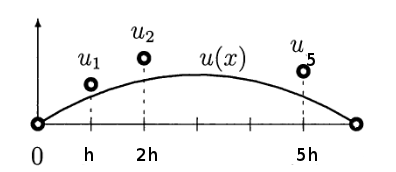
\includegraphics[height=4cm]{2_6.png}

$K$ matrisinin 5x5 olmasi karisiklik yaratmis olabilir. Burada sebep K
matrisine $u_0$ ve $u_6$'nin dahil edilmemis olmasi, cunku o degerleri
zaten biliyoruz. Bu degerler olsaydi $K$ matrisinin sol ve sagina tamamen
sifir iceren iki kolon gerekecekti, $u$ vektorune alttan ve ustten $u_0$ ve
$u_6$ eklenecekti ve bu iki deger sifir oldugu icin $K$'nin sol ve
sagindaki sifirlar ile carpilacaklardi, bu yuzden mevcut toplam uzerinde
hic etkileri olmayacakti . Bu sebeple bu iki kolonu ve $u$ degerini tamamen
kaldirmak sonuc uzerine hicbir etki yapmiyor.

Devam edelim. Simdi orijinal problemi degistirelim. Eger ustteki problem
iki ucu sabitlenmis kendi agirligiyla asilan bir elastik cubugu
gosteriyorsa (ve $u$ degerleri cubugun ne kadar uzadigini temsil ediyorsa),
bu sefer ustteki ucu serbest birakabiliriz. Yani $u(0)=0$ olmayacak.

Yine birbicimli (uniform) cubuk, esit dagilmis yuk. 

\[ -\frac{d^2u}{dx^2} = 1 \]

\[ \frac{du}{dx}(0) = 0, \ u(1) = 0 \]

Burada ilk sart $u$'nin egiminin (slope) sifira esitlenmis olmasi.

Onceki denklemdeki genel cozum hala ise yarar. 

\[ u(x) = -\frac{1}{2}x^2 + Cx + D\]

\[ \frac{du}{dx} = -x + C \]

\[ \frac{du}{dx}(0) = 0 + C = 0 \]

\[ C = 0 \]

\[ u(1) = 0 = -1/2 + 0 + D  \]

\[ D = 1/2  \]

O zaman cozum

\[ u(x) = -\frac{1}{2}x^2  + 1/2\]


Grafikleyince suna benzer

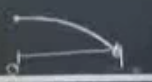
\includegraphics[height=2cm]{2_4.png}

Egimin sifir noktasinda sifir oldugunu goruyoruz. 

Simdi farkliliklar formulune gelelim. Diferansiyel denklemin karsiligi olan
farklilik formulu nedir? Hala ayni:

\[ \frac{-u_{i+1}+2u_i - u_{i-1}}{h^2} = f(x_i)\]

Simdi onemli noktaya geldik: baslangic sartlari ne olacak? $u(1)=0$ kolay,
$ du/dx(0) = 0$ nasil temsil edilecek? Bir fikir su olabilir. 

\[ \frac{u_1-u_0}{h} = 0 \]

Bu ifadeyi matrise nasil tercume ederiz? Ustteki ifade ayni zamanda $u_1 -
u_0 = 0$ demektir, yer degistirince $u_1 = u_0$. $K$ matrisinin birinci
satiri nedir?

\[ -u_0 + 2u_1 - u_2 \]

$u_0$ yerine $u_1$ koyalim

\[ = -u_1 + 2u_1 - u_2 \]

\[ = u_1 - u_2 \]

O zaman birinci satiri ustteki gibi degistirirsek, s�n�r sartlarindan
birini yerine getirmis oluruz, yani ilk satira [1 -1] koyacagiz, orada
[2 -1] yerine [1 -1] var artik. Matris bu sekilde degisince ona $K$ yerine
$T$ matrisi deniyor. $TU = [1, 1, ...]$.

\[ 
\frac{1}{h^2}
\left[\begin{array}{rrrrr}
1 & -1 & & & \\
-1 & 2 & -1 & & \\
& -1 & 2 & -1 & \\
& & -1 & 2 & -1 \\
& & & -1 & 2
\end{array}\right]
\left[\begin{array}{r}
u_1 \\
u_2 \\
u_3 \\
u_4 \\
u_5 
\end{array}\right] 
=
\left[\begin{array}{r}
1 \\
1 \\
1 \\
1 \\
1 
\end{array}\right]
 \]


Soru: ayriksal cozum gercek cozume ne kadar yakin? Cevap hata payi $O(h)$
cunku $(u_1 - u_0) / h$ tan�m� birinci dereceden bir yakla��ksall�k
(approximation). Kabaca cizince soyle gozukur:

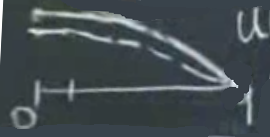
\includegraphics[height=2cm]{2_7.png}

Hesap kalitesi pek iyi denemez. Cozumu ikinci dereceden yapsak daha iyi
olacakti. Nasil? $(u_1 - u_0) / h$ yerine baska bir sey kullanmamiz
lazim. Ortalanmis farkliligi hatirlayalim, bu yontem ikinci derece
dogrulugu olan bir yontemdir, 

Problem 1.2 A

Kitaptaki ufak problemi hatirlayalim

\[ 
\left[\begin{array}{rrr}
1 & -1 & \\
-1 & 2 & -1 \\
& -1 & 2
\end{array}\right]
\left[\begin{array}{r}
u_1 \\
u_2 \\
u_3 
\end{array}\right] 
=
\left[\begin{array}{r}
1 \\
1 \\
1 
\end{array}\right]
 \]

Bu problem iste $O(h)$ hatasini azaltma konusunu
isliyor, bunun icin ortalama farklilik (centered difference) kullanilacak,
$(u_1 - u_o)/h$ yerine 0'�nc� degere denk gelecek sekilde farkliligi
ortalayacagiz, 0 uzerinde ortalama yapmamiz icin onun bir gerisine ve bir
ilerisine gitmek lazim, o zaman once $K$ matrisini bir genisletelim, cunku
artik $u_0$'in dahil edilmesi gerekecek ve hayali bir $u_{-1}$'i dusunelim,
$u'(0) =
0$ icin 

\[ \frac{u_1-u_{-1}}{2h} = 0\]

tanimini kullanalim. O zaman

\[ u_1 - u_{-1} = 0\]

\[ u_1 =  u_{-1} \]

\[ -u_{-1} + 2u_0 - u_1 = h^2 f(0) \]

$u_1 =  u_{-1}$ ifadesini yerine koyalim

\[ -u_1 + 2u_0 - u_1 = h^2 f(0) \]

\[ -2u_1 + 2u_0 = h^2 f(0) \]

\[ -u_1 + u_0 = \frac{1}{2} h^2 f(0) \]

O zaman matrisin ust sol degeri $u_0$ katsayisina gore 1, onun sagindaki
deger $u_1$ katsayisina gore -1 olmali. $1/2$ degerini de esitligin
sagindaki $f$ icin kullandigimiza dikkat. Tum bunlari $u_{-1}$'in yerine
deger gecirerek elde ettigimiz icin o kolona artik ihtiyac kalmadi, o
gecici kolon, matristen atildi. 

\[ \frac{1}{h^2}
\left[\begin{array}{rrrr}
1 & -1 & & \\
-1 & 2 & -1 & \\
& -1 & 2 & -1 \\
 & & -1 & 2
\end{array}\right]
\left[\begin{array}{r}
u_0 \\
u_1 \\
u_2 \\
u_3 
\end{array}\right] 
=
\left[\begin{array}{r}
1/2 \\
1 \\
1 \\
1 
\end{array}\right]
 \]

Matris boyutlarinin nasil buyudugune, ve $u_0$'in dahil edilmesine dikkat
edelim. Problemin basindaki matris 3x3 boyutundaydi, bu 4x4 boyutunda,
ayrica $h$ hala $1/4$ degerinde. 

Problem 1-2-A

\begin{minted}[fontsize=\footnotesize]{python}
import scipy.linalg as lin

def ktbc(n):
    vec = np.zeros((1,n))
    vec[0,0] = 2
    vec[0,1] = -1
    K = lin.toeplitz(vec)
    T = np.copy(K)
    T[0,0] = 1
    B = np.copy(K)
    B[0,0] = 1
    B[n-1,n-1] = 1
    C = np.copy(K)
    C[n-1,n-1] = 1
    
    return K, T, B, C

K,T,B,C = ktbc(3); print T

h = 1./4.

discrete = lin.solve( (1./h)**2 * T, [1.,1.,1.] )

discrete = np.insert(discrete, 0, discrete[0]) 
discrete = np.append(discrete, 0.) 

K,T,B,C = ktbc(4); print T

discrete_2 = lin.solve( (1./h**2)*T, [1./2.,1.,1.,1.] )
# add little diff for plotting
# grafik ust uste binmesin diye azicik fark ekledik
discrete_2 = discrete_2 + 0.01 
discrete_2 = np.append(discrete_2, 0.) 

def u(x): return (1./2.)*(1. - x**2)

p1 = plt.plot([u(0.0), u(0.25), u(0.5), u(0.75), u(1.)])

p2 = plt.plot(discrete)

p3 = plt.plot(discrete_2)

plt.legend([p1,p2,p3], ["analytical solution (analitik cozum)",
                        "discrete solution 1 (ayriksal cozum 1)",
                        "discrete solution 2 (ayriksal cozum 2)"
                        ])

plt.savefig('1-2-A.png')
\end{minted}

\begin{verbatim}
[[ 1. -1.  0.]
 [-1.  2. -1.]
 [ 0. -1.  2.]]
[[ 1. -1.  0.  0.]
 [-1.  2. -1.  0.]
 [ 0. -1.  2. -1.]
 [ 0.  0. -1.  2.]]
\end{verbatim}

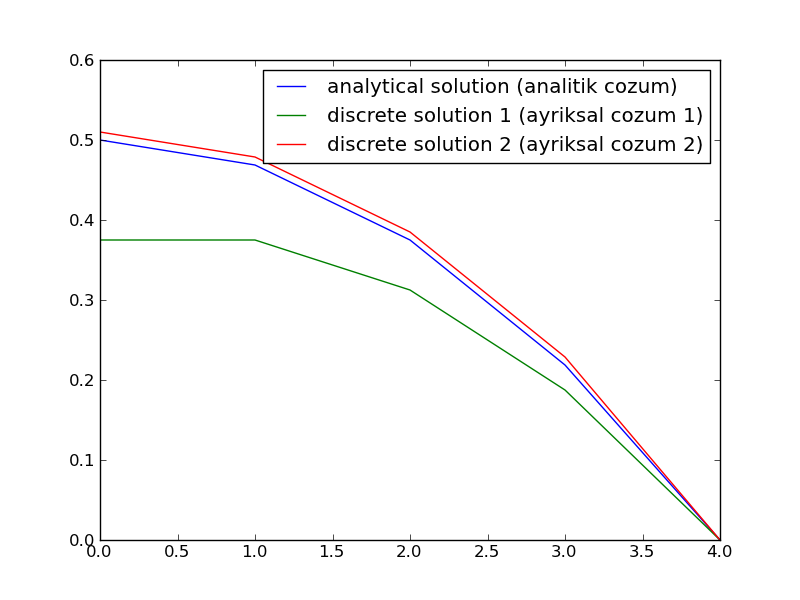
\includegraphics[height=6cm]{1-2-A.png}

Guzel. Artik hesap gercek sonuca iyice yaklasacak. 

[Derse donelim] Bunlardan bahsetmemizin onemli bir sebebi s�n�r sartlarinin
ne kadar onemli oldugunu anlatmak. Goruldugu gibi s�n�r sartlari, onlarin
yaklasiksallanma yontemleri sonucun uzerinde direk bir etki yaratiyor.

Bir dipnot olarak bahsedelim, burada kullandigimiz metot s�n�rl�
farkliliklar (finite differences) metodu. Eger s�n�rl� elementler (finite
elements) metodu kullaniyor olsaydik, ustteki satirin degismesi otomatik
olarak gerceklesecekti. S�n�rl� elementler metotu ileriki derslerin birinde
islenecek.

Soru 1.2.7

Bu soruda $u$'dan alinacak dort veri noktasiyla (sample) $du/dx$ ortada
olmak uzere 4. seviye kesinlik elde edilebilecegi soyleniyor. 

\[ \frac{-u_2 + 8u_1 - 8u_{-1} + u_{-2}}{12h} = \frac{du}{dx} + bh^4
\frac{d^5}{dx^5} + ..\]

Bu problemin tum cebirsel cozumu Ingilizce ders notlarinda. Ek aciklama
olarak sunu ekleyelim: Esitligin sol tarafindaki 1, 8 gibi katsayilar
modelleyici tarafindan secilmis, bir teorinin, ispatin sonucu degil. Hala
birincil farklilik (first differences) dunyasindayiz, ama ileri, geriye
gidip katsayi 1 kullanmak yerine dort noktayi kullanmak istemis, ve
ortadaki noktalara daha fazla ``agirlik'' vermek istemisiz. Tabii bu
katsayilarla bu noktalar kullanilinca, ortalamanin duzelmesi icin
katsayilarin bolume yansimasi gerekiyor, o yuzden bolumde $12h$ goruyoruz.

Ve aynen ileri, geriye dogru ayriksal formu surekli fonksiyonlar uzerinde
Taylor serisiyle temsil edebildigimiz gibi, ustteki esitligin sol tarafini
da Taylor serisi ile $u(x+h)$ turu terimler uzerinden temsil
edebiliriz. Ustte $u_{2}$, $u_{-1}$ gibi ibareler var, bunlarin Taylor
karsiligi $u(x+2h)$, $u(x-h)$ gibi ifadeler olur. Katsayi carpimlarinin ve
$12h$'ye bolum isleminin Taylor serisi uzerinde de aynen kullanilmasi
gerekiyor tabii ki. 

Bu arada $b$ sabitinin ne oldugunu soru soylemiyor, ama tum bu cebirsel
islemi gerceklestirince denklemdeki esitligin sag tarafi aynen elde
edilecek ve boylece $b$ yerine hangi sayi gelecegi de ortaya cikacak.

\end{document}
